\documentclass[12pt]{article} 
\usepackage[left=14mm, top=16mm, right=16mm, bottom=20mm]{geometry} 
\usepackage{graphicx}
\usepackage{wrapfig}
\graphicspath{{../pictures/}}
\DeclareGraphicsExtensions{.pdf,.png,.jpg,.eps}
\usepackage{cmap}					% поиск в PDF
\usepackage{mathtext} 				% русские буквы в формулах
\usepackage[T2A]{fontenc}	
\usepackage[utf8x]{inputenc} 
\usepackage[russian]{babel} 
\usepackage{amsmath,amsfonts,amssymb,amsthm,mathtools} 
\usepackage{icomma} % "Умная" запятая: $0,2$ --- число, $0, 2$ --- перечисление
\usepackage{euscript}	 % Шрифт Евклид
\usepackage{mathrsfs} % Красивый матшрифт
\usepackage{indentfirst}     % Отступ в первом абзаце
% Перенос знаков в формулах (по Львовскому)
\newcommand*{\hm}[1]{#1\nobreak\discretionary{}
	{\hbox{$\mathsurround=0pt #1$}}{}}

%% Свои команды
%DeclareMathOperator{\sgn}{\mathop{sgn}}
%\newcommand{\te}{\ensuremath{\Rightarrow}}
%\newcommand{\y}{\ensuremath{\angle}}
%\newcommand{\ABC}{\ensuremath{\triangle ABC\,}}
%\newcommand{\tr}{\ensuremath{\triangle}}
%\newcommand{\ca}{\ensuremath{\cos\alpha}}
%\newcommand{\sa}{\ensuremath{\sin\alpha}}
%\newcommand{\cb}{\ensuremath{\cos\beta}}
%\newcommand{\sib}{\ensuremath{\sin\beta}}
%\newcommand{\ov}{\ensuremath{\overline}}
%\newcommand{\x}{\cdot}
%\newcommand{\de}{\varDelta}
%\newcommand{\st}{\ensuremath{\longrightarrow}}
%DeclareMathOperator{\Sum}{\mathop{Sum}}
%\DeclareMathOperator{\Sum}{\mathop{Sum}}

\begin{document}
	
\begin{titlepage}		
\begin{center}
\large 	Московский физико-технический университет \\
Факультет общей и прикладной физики \\
\vspace{0.2cm}
Учебная программа\\
"<Квантовая теория поля, теория струн и математическая физика">

\vspace{4.5cm}
II семестр 2016-2017 учебного года \\ \vspace{0.1cm}
\large Домашнее задание №5: \\ \vspace{0.1cm}
\LARGE \textbf{Специальная теория относительности}
\end{center}
\vspace{2.3cm} \large

\begin{center}
		 Автор: \\
 Иванов Кирилл,
 625 группа
\vspace{10mm}


\end{center}

\begin{center} \vspace{50mm}
г. Долгопрудный \\ 
8 мая 2017 года
\end{center}
\end{titlepage}

%______________________________________________________________________________________________

\section{Вопрос №1}

 \begin{wrapfigure}{l}{0.4\linewidth} 
	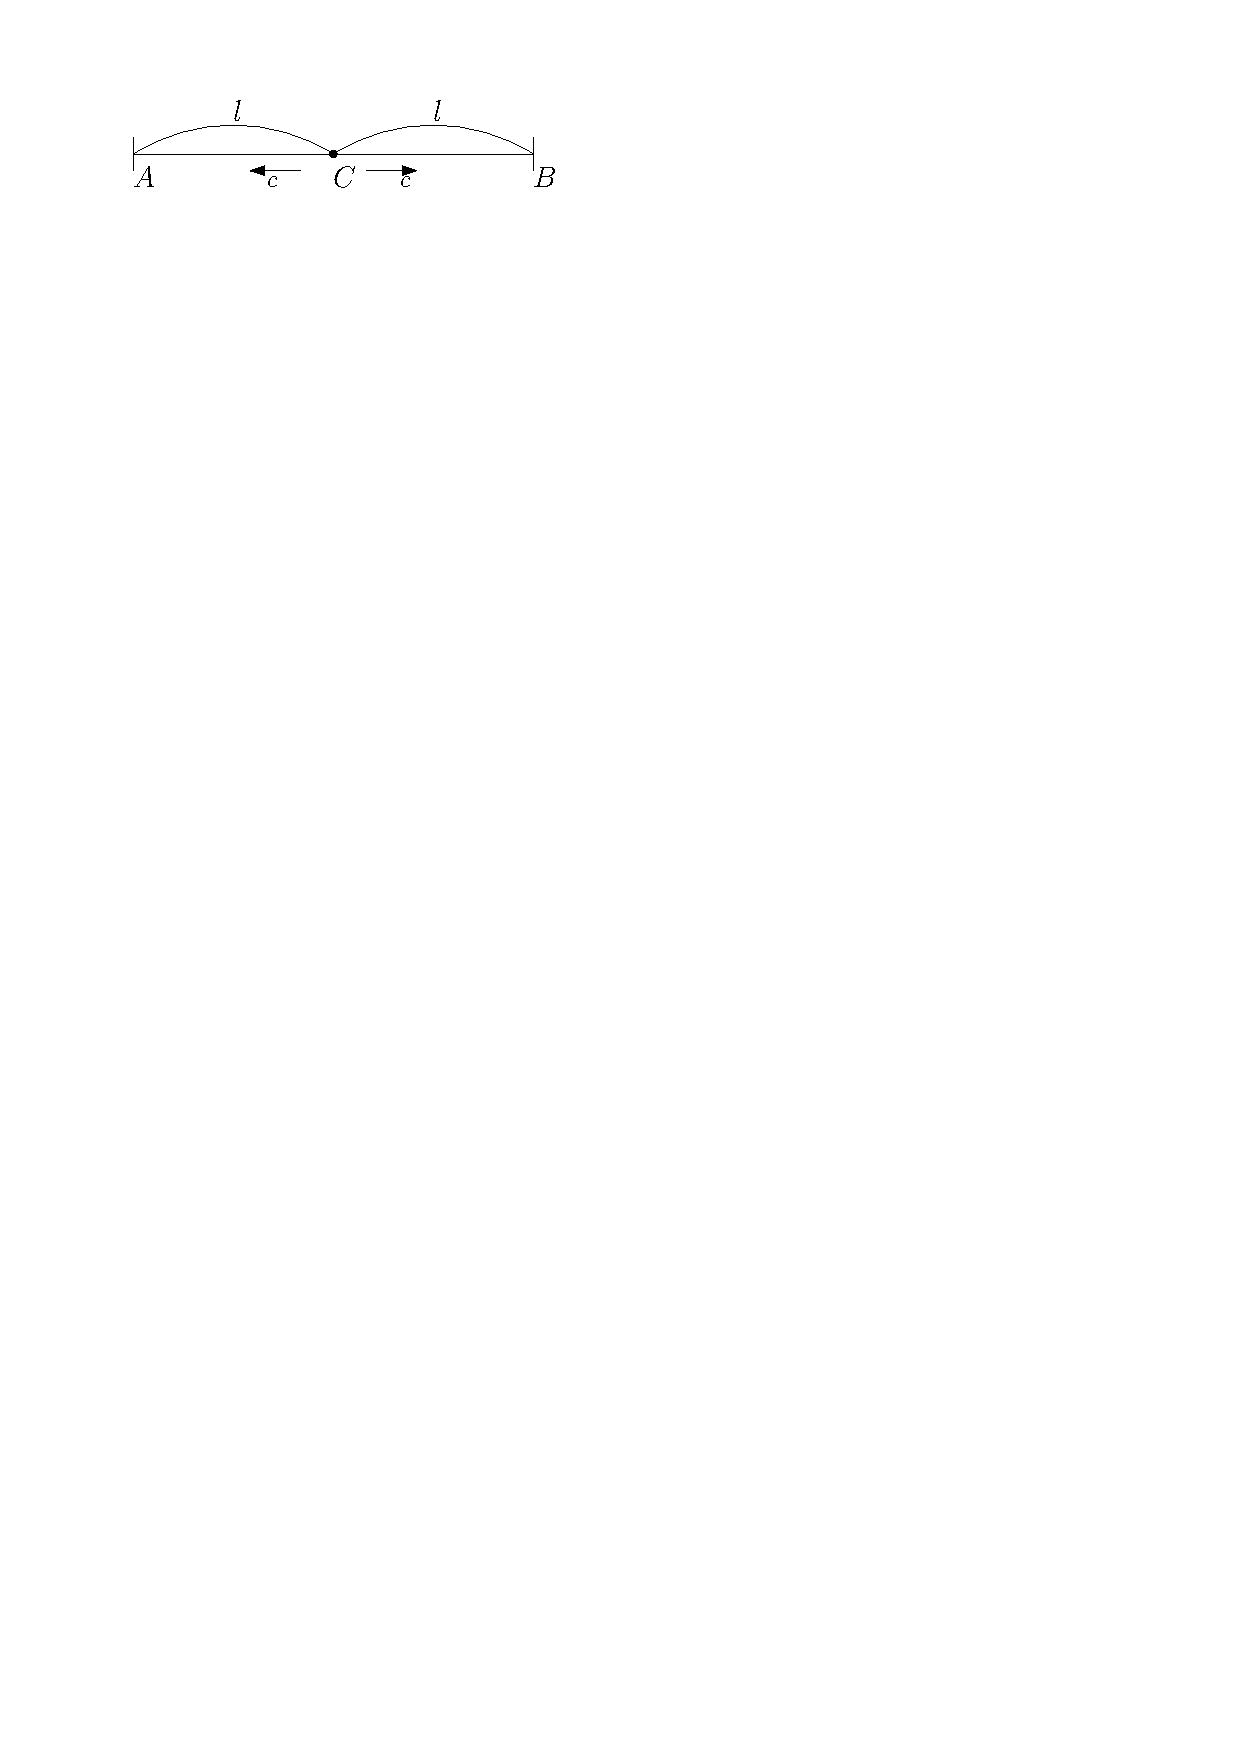
\includegraphics{5_1f}
	\caption{Синхронизация часов}
\end{wrapfigure}

Поскольку скорость света конечна, возникает проблема синхронизации часов в каждой из двигающихся различных образующих систем. Вместо \textit{абсолютного времени} возникает \textit{местное время}. 

Ввиду того, что из принципа относительности скорость света в каждой инерциальной системе отсчета равна $ c $, возникает естественный способ синхронизации часов, предложенный Эйнштейном. 

Рассмотрим часы, находящие в точках $ A $ и $ B $  отрезка длиной $ 2l $. Из точки $ С  : AC = CB = l $ пустим световой луч, движущийся со скоростью $ c $. Тогда часы будут называться \textbf{синхронными} в инерциальной системе $ K $, если этот луч дойдет до них в  одинаковый момент по их показаниям.

\section{Задача  №1}

 \begin{wrapfigure}{l}{0.45\linewidth} 
	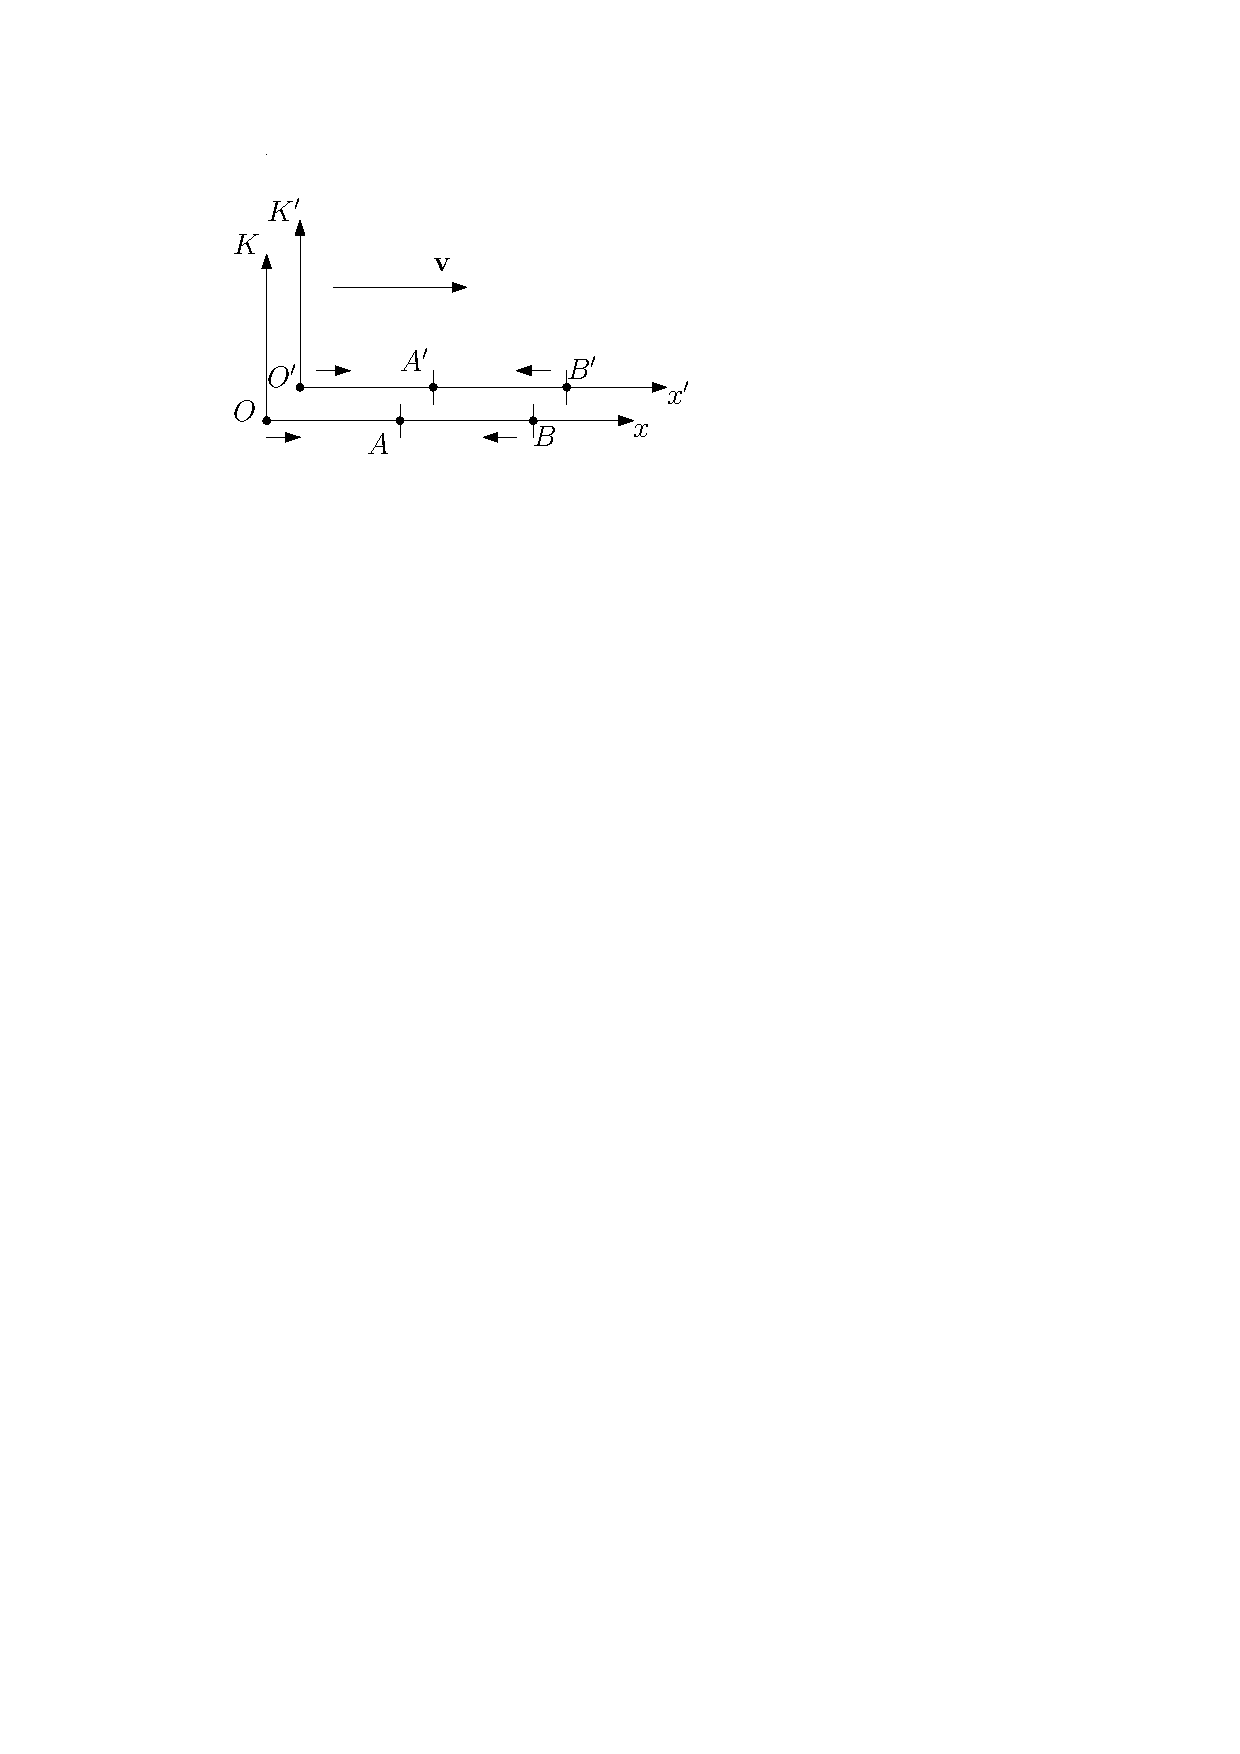
\includegraphics{5_2}
	\caption{Разность показания часов}
\end{wrapfigure}

Итак, по условию задачи в системе $ K $ в момент времени $ t = 0 $ из точек $ O $ и $ B $ вылетают 2 световых луча, которые встречаются в точке $ A $. Аналогичные условия и обозначения для $ K' $ Координата $ B = (x), A = (\frac{x}{2}). $ Тогда понятно, что в системе $ K $ наши лучи встретятся в момент времени $ t= \dfrac{x}{2c}. $

Очевидно, что наблюдатель, сидящий в точке $ A' $ в системе $ K' $ увидит луч, вылетевший из $ В' $ раньше, чем тот, что вылетел из $ O' $ (действительно, ведь он движется навстречу $ B' $ со скоростью $ V $ и удаляется от $ O' $ с той же скоростью). Т.е. если мы обозначим время встречи с первым и вторым лучами за $ t_1', t_2' $ соответственно, то $ t_1' \neq t_2' $. 

Из второго постулата СТО, свет в системе $ K' $ движется со скоростью $ c $ (как и в любой другой ИСО). Понятно, что $ O'A' = c\tau, $ где $ \tau $ --- время встречи лучей в системе $ K' $ (мы считаем, что в движущейся системе лучи также встретились в середине отрезка $ O'B' $ в силу 1 постулата СТО, при это разница относительно $ K $ достигается за счёт неодновременности  выпуска лучей). Однако путь, пройденный левым сигналом, равен $ O'A' = \dfrac{x'}{2} + V\tau = c\tau. $

Обозначим за $ \de t' $ время, в момент которого свет испускается из точки $ B' $, и понятно, что это и есть искомое время разности часов. Тогда из аналогичных соображений $ O'B' = \dfrac{x'}{2} - V(\tau - \de t') = с(\tau - \de t') $.  Запишем систему:

\begin{equation}
\left\{
\begin{aligned}
&\dfrac{x'}{2} + V\tau = c\tau \\
&\dfrac{x'}{2} - V(\tau - \de t') = с(\tau - \de t') \\
& x' = x\sqrt{1 - v^2/c^2} \text{ (Релятивистское сокращение длины)}
\end{aligned}
\right.
\end{equation}

Решая эту систему, мы получаем: 

\begin{equation}
\de t' = \dfrac{Vx'}{c^2 - v^2} = \dfrac{Vx\sqrt{c^2-v^2}}{c(c^2 - v^2)} =  \dfrac{Vx}{c^2\sqrt{1 - v^2/c^2}}.
\end{equation}

\begin{center}
	{\fbox{Ответ: $ \de t' = \dfrac{Vx}{c^2\sqrt{1 - v^2/c^2}} $}} \\
\end{center} 

\section{Задача №2}

 \begin{wrapfigure}{l}{0.3\linewidth} 
	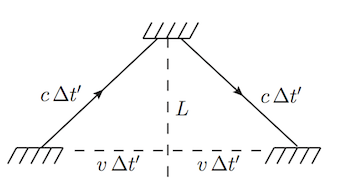
\includegraphics{5_3.png}
	\caption{Растяжение времени}
\end{wrapfigure}

Понятно, что в покоящейся системе $ К $ время пробега $ \tau = 2\de t = \frac{2L}{c}. $ Однако в движущейся $ K' $ это не так, и $ \tau' = 2\de t' \neq \tau. $

Дело в том, что хотя часы проходят, конечно, расстояние $ 2c\de t' $, оно не равно расстоянию $ 2L $. За время $ \de t' $  часы смещаются на расстояние $ V\de t' $ по направлению движения стержня, ну а по вертикали наш сигнал смещается, естественно, на $ L $ (см. рисунок). Тогда можно записать теорему Пифагора:

\begin{equation}
c^2\de t'^2 = v^2\de t'^2 + L^2 
\end{equation}
$$ 
(c^2 -v^2) \de t'^2 = L^2
$$
$$
\de t' = \dfrac{L}{\sqrt{c^2-v^2}}
$$

Учитывая  $ \tau' = 2\de t'$, получаем ответ:
\begin{center}
	{\fbox{Ответ: $ \tau' = \dfrac{2L}{c\sqrt{1-v^2/c^2}} = \dfrac{\tau}{\sqrt{1-v^2/c^2}}$}} \\
\end{center} 

\section{Задача №3}

 \begin{wrapfigure}{l}{0.4\linewidth} 
	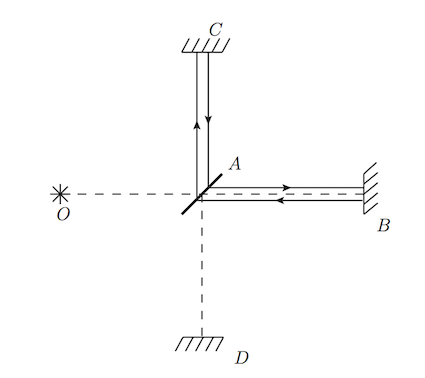
\includegraphics{5_4.png}
	\caption{Опыт Майкельсона-Морли}
\end{wrapfigure}

Рассмотрим опыт Майкельсона-Морли. В движущейся системе $ K' $ рассмотрим движение света от зеркала $ А $ к $ В $ и $ С $ соответственно.

Понятно, что при движении в горизонтальном направлении время между уходом сигнала из точки А в В и приходом обратно равно 
\begin{equation}
\tau_г = \dfrac{AB}{c + v} + \dfrac{AB}{c - v}
\end{equation}

А при движении в вертикальном направлении происходит смещение часов, и согласно задаче №2, 

\begin{equation}
\tau_в = \dfrac{2AC}{\sqrt{c^2-v^2}}
\end{equation}

Из первого постулата СТО следует, что в системе $ K' $ должны происходить те же явления, что и в $ K \te \tau_в = \tau_г $. Так мы получаем:

\begin{equation}
AB\dfrac{2c}{c^2 - v^2} = \dfrac{2AC}{\sqrt{c^2-v^2}} \te AB = AC\sqrt{1-v^2/c^2}
\end{equation}

Если в системе $ K \hookrightarrow AB = AC = L$, то в системе $ K' $ происходит сокращение Лоренца-Фицжеральда.

\begin{center}
	{\fbox{Ответ: $ L' = L \sqrt{1-v^2/c^2}$}} \\
\end{center} 

\section{Задача №4}

 \begin{wrapfigure}{l}{0.34\linewidth} 
	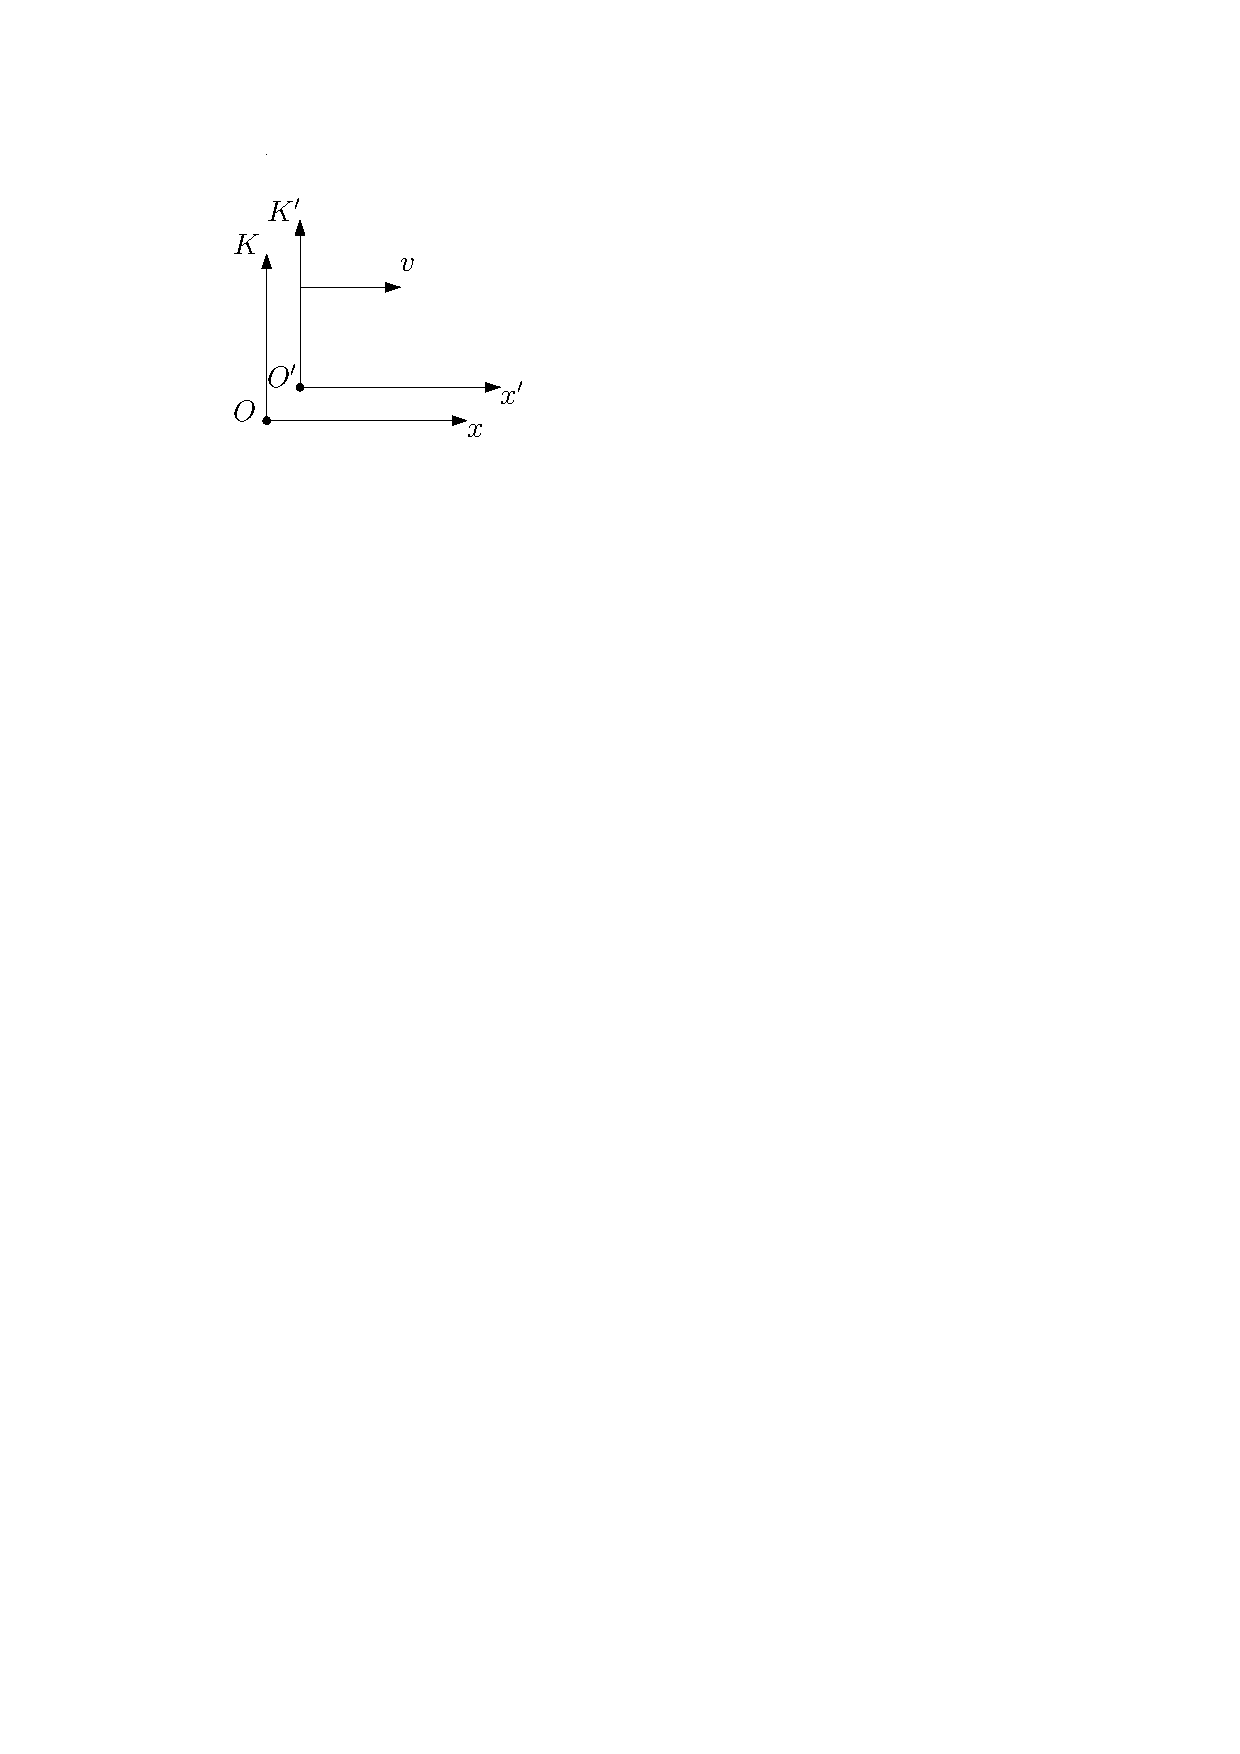
\includegraphics{5_5}
	\caption{Движение ИСО}
\end{wrapfigure}

В нерелятивистском случае ($ v \ll c $) верны преобразования Галлилея:

\begin{equation}
\left\{
\begin{aligned}
& x' = x + vt' \\
& t =t' \\
\end{aligned}
\right.
\end{equation}

Когда скорость движения $ K' $ сравнима со скоростью света, они переходят в преобразования Лоренца. 

Как было показано в задаче №3, $ x \st x\sqrt{1-v^2/c^2}  $, а из задачи №2 $ t \st \dfrac{t}{\sqrt{1-v^2/c^2}}. $ Кроме того, появляется эффект относительности одновременности, или же "<отставание часов">: $ \de t' = \dfrac{Vx}{c^2\sqrt{1 - v^2/c^2}} $, который добавляется ко времени $ t' $

Так мы приходим к искомым преобразованиям Лоренца: 

\begin{equation}
\left\{
\begin{aligned}
& x' = x\sqrt{1-v^2/c^2} + vt' \\
& t = \dfrac{t}{\sqrt{1-v^2/c^2}} + \dfrac{Vx}{c^2\sqrt{1 - v^2/c^2}} \\
\end{aligned}
\right.
\end{equation}

Преобразуем и выразим все через "<нештрихованные"> координаты:

\begin{equation}
\left\{
\begin{aligned}
&x' = \dfrac{x + vt}{\sqrt{1-v^2/c^2}} \\
&t' = \dfrac{t + vx/c^2}{\sqrt{1-v^2/c^2}} \\
\end{aligned}
\right.
\end{equation}

Это и есть искомые преобразования Лоренца.




\end{document}